

\documentclass{beamer}

\usepackage{xcolor}
\definecolor{blackl}{RGB}{12,14,18}

\usetheme{Warsaw} %Berkeley Goettingen Hannover Berlin
\setbeamercolor{normal text}{fg=white,bg=blackl}
\setbeamercolor{structure}{fg=white}

\setbeamercolor{alerted text}{fg=red!85!black}

\setbeamercolor{item projected}{use=item,fg=black,bg=item.fg!35}

\setbeamercolor*{palette primary}{use=structure,fg=structure.fg}
\setbeamercolor*{palette secondary}{use=structure,fg=structure.fg!95!black}
\setbeamercolor*{palette tertiary}{use=structure,fg=structure.fg!90!black}
\setbeamercolor*{palette quaternary}{use=structure,fg=structure.fg!95!black,bg=black!80}

\setbeamercolor*{framesubtitle}{fg=white}

\setbeamercolor*{block title}{parent=structure,bg=black!60}
\setbeamercolor*{block body}{fg=black,bg=black!10}
\setbeamercolor*{block title alerted}{parent=alerted text,bg=black!15}
\setbeamercolor*{block title example}{parent=example text,bg=black!15}

\usepackage{german}


\begin{document}

\title{OpenCV}   
\author{Florian Herrmann} 
\date{\today}
\logo{
\includegraphics[scale=0.3]{Bilder/HAWK_Logo.jpg} 
\includegraphics[scale=0.15]{Bilder/OpenCV.png}}

\begin{frame}
\titlepage
\end{frame}

\section{Namensgebung \& Historie}
\begin{frame} \frametitle{Namensgebung}
	$Open + Computer Visson = OpenCV$
	
\end{frame}

\begin{frame} \frametitle{Historie}
	\begin{itemize}
		\item [2000]
	
	\end{itemize}
	\cite{GitHub}
\end{frame}

\begin{frame} \frametitle{Projektidee}
	Programiert in C++ (Laufzeit optimiert)
	\begin{figure}
		\centering
		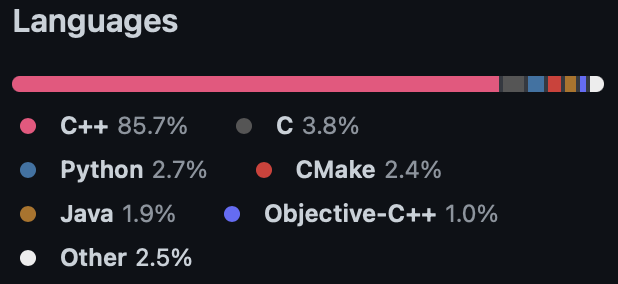
\includegraphics[width=0.85\textwidth]{Bilder/CodeBase.png}
		\label{a4}
	\end{figure}
\end{frame}

\begin{frame} \frametitle{Projektidee}
	Zur Verwendung eines Schmidt-Cassegrain-Teleskop in  einem Kleinstsatelliten soll dieses in einer monolithischen Anordnung umgesetzt werden.\\
	\textbf{Dies bietet folgen Vorteile:}\\
	\begin{itemize}
		\item  Durch die geringe  Wärmeausdehnung des Glases, ist ein solcher Aufbau weniger anfällig für thermische Ausdehnung. \pause
		\item Der Aufbau ist resilient gegenüber  Schlägen und Vibration.
	\end{itemize}
\end{frame}

\section{Material und Größe}
\begin{frame}
	\frametitle{Material und Größe}
	Randbedingungen für den Aufbau:
		\begin{itemize}
		\item  Material: NBK7 von der Firma Schott \pause
		\item Apertur: $\varnothing 30 ~mm$ \pause
		\item Länge: $ 34 ~mm$ \pause
		\item Wellenlängenbereich: $\lambda_1 = 486~nm $ bis $ \lambda_3=656 ~nm$ \pause
		\item Maximales Gesamtgewicht des  Satelliten: $ 1.3 ~kg$ \pause
		\item Maximales Kantenlänge des  Satelliten: $ 100 ~mm$ 
	\end{itemize}
\end{frame}


\section{Simulation}

\begin{frame}\frametitle{Simulation}
	\textbf{Vorgehen:}
	\begin{itemize}
		\item Eintragen der Apertur und der Wellenlängen. \pause
		\item Eintragen der Flächen und deren Aperturen. \pause
		%\item Überprüfen des Strahlengangs. \pause
		\item Automatic Designer mit Randbedingungen \glqq füttern\grqq. \pause 
	\end{itemize}

\end{frame}

\begin{frame}\frametitle{Simulation}
\textbf{Vorgehen:}
	\begin{itemize}
		\item Eintragen der Apertur und der Wellenlängen. 
		\item Eintragen der Flächen und deren Aperturen. 
		%\item Überprüfen des Strahlengangs. \pause
		\item Automatic Designer mit Randbedingungen \glqq füttern \grqq. 
	\end{itemize}

\end{frame}




\section{Ergebnisse}
\begin{frame}
	\frametitle{Ergebnisse}

 \begin{itemize}
 	\item Auflösungsvermögen: $230 ~\frac{Linienpaare}{mm}  \approx 2,17~\mu m$\pause
 	\item RMS-Radius:  $0,003118~mm$ \pause
 	\item Vergrößerung: $V=3,14 $  \pause
 	\item Auflösung: $A=(4,54\pm0,7)~m$\pause
 	\item Gewicht: $m = 151.4~g$ \pause
 	\item Länge: $l =  62 ~mm$
 	 
 \end{itemize}
\end{frame}



\section[Quellen]{Referenzen}
\begin{frame}\frametitle{Quellen \& Literatur}

	\begin{thebibliography}{9}
		
		\bibitem{GitHub} 
		GitHub: OpenCV
		\\\texttt{Open Source Computer Vision Library}
		\url{https://github.com/opencv/opencv}
		[abgerufen am: 21.05.2022]
		
		\bibitem{Bradski2008}
		Bradski, A. Learning OpenCV - Computer Vision with the OpenCV Library. (OReilly Media, Inc. ,2008)
		
		
		
		
		
	\end{thebibliography}

\end{frame}


\begin{frame}
	\frametitle{Ergebnisse}
	

\begin{minipage}{0.45\textwidth}
		\begin{equation}
			1,22\cdot\dfrac{\lambda}{d}=\theta_{min}~(rad)	
		\label{f2}
	\end{equation}
\end{minipage}
\begin{minipage}{0.1\textwidth}
\end{minipage}
\begin{minipage}{0.45\textwidth}
	\begin{equation}
	A=2\cdot\sin\left(\frac{\theta_{min}}{2}\right)\cdot h	~~.
	\label{f3}
	\end{equation}
\end{minipage}
\end{frame}

\end{document}
